\documentclass[1p]{elsarticle_modified}
%\bibliographystyle{elsarticle-num}

%\usepackage[colorlinks]{hyperref}
%\usepackage{abbrmath_seonhwa} %\Abb, \Ascr, \Acal ,\Abf, \Afrak
\usepackage{amsfonts}
\usepackage{amssymb}
\usepackage{amsmath}
\usepackage{amsthm}
\usepackage{scalefnt}
\usepackage{amsbsy}
\usepackage{kotex}
\usepackage{caption}
\usepackage{subfig}
\usepackage{color}
\usepackage{graphicx}
\usepackage{xcolor} %% white, black, red, green, blue, cyan, magenta, yellow
\usepackage{float}
\usepackage{setspace}
\usepackage{hyperref}

\usepackage{tikz}
\usetikzlibrary{arrows}

\usepackage{multirow}
\usepackage{array} % fixed length table
\usepackage{hhline}

%%%%%%%%%%%%%%%%%%%%%
\makeatletter
\renewcommand*\env@matrix[1][\arraystretch]{%
	\edef\arraystretch{#1}%
	\hskip -\arraycolsep
	\let\@ifnextchar\new@ifnextchar
	\array{*\c@MaxMatrixCols c}}
\makeatother %https://tex.stackexchange.com/questions/14071/how-can-i-increase-the-line-spacing-in-a-matrix
%%%%%%%%%%%%%%%

\usepackage[normalem]{ulem}

\newcommand{\msout}[1]{\ifmmode\text{\sout{\ensuremath{#1}}}\else\sout{#1}\fi}
%SOURCE: \msout is \stkout macro in https://tex.stackexchange.com/questions/20609/strikeout-in-math-mode

\newcommand{\cancel}[1]{
	\ifmmode
	{\color{red}\msout{#1}}
	\else
	{\color{red}\sout{#1}}
	\fi
}

\newcommand{\add}[1]{
	{\color{blue}\uwave{#1}}
}

\newcommand{\replace}[2]{
	\ifmmode
	{\color{red}\msout{#1}}{\color{blue}\uwave{#2}}
	\else
	{\color{red}\sout{#1}}{\color{blue}\uwave{#2}}
	\fi
}

\newcommand{\Sol}{\mathcal{S}} %segment
\newcommand{\D}{D} %diagram
\newcommand{\A}{\mathcal{A}} %arc


%%%%%%%%%%%%%%%%%%%%%%%%%%%%%5 test

\def\sl{\operatorname{\textup{SL}}(2,\Cbb)}
\def\psl{\operatorname{\textup{PSL}}(2,\Cbb)}
\def\quan{\mkern 1mu \triangleright \mkern 1mu}

\theoremstyle{definition}
\newtheorem{thm}{Theorem}[section]
\newtheorem{prop}[thm]{Proposition}
\newtheorem{lem}[thm]{Lemma}
\newtheorem{ques}[thm]{Question}
\newtheorem{cor}[thm]{Corollary}
\newtheorem{defn}[thm]{Definition}
\newtheorem{exam}[thm]{Example}
\newtheorem{rmk}[thm]{Remark}
\newtheorem{alg}[thm]{Algorithm}

\newcommand{\I}{\sqrt{-1}}
\begin{document}

%\begin{frontmatter}
%
%\title{Boundary parabolic representations of knots up to 8 crossings}
%
%%% Group authors per affiliation:
%\author{Yunhi Cho} 
%\address{Department of Mathematics, University of Seoul, Seoul, Korea}
%\ead{yhcho@uos.ac.kr}
%
%
%\author{Seonhwa Kim} %\fnref{s_kim}}
%\address{Center for Geometry and Physics, Institute for Basic Science, Pohang, 37673, Korea}
%\ead{ryeona17@ibs.re.kr}
%
%\author{Hyuk Kim}
%\address{Department of Mathematical Sciences, Seoul National University, Seoul 08826, Korea}
%\ead{hyukkim@snu.ac.kr}
%
%\author{Seokbeom Yoon}
%\address{Department of Mathematical Sciences, Seoul National University, Seoul, 08826,  Korea}
%\ead{sbyoon15@snu.ac.kr}
%
%\begin{abstract}
%We find all boundary parabolic representation of knots up to 8 crossings.
%
%\end{abstract}
%\begin{keyword}
%    \MSC[2010] 57M25 
%\end{keyword}
%
%\end{frontmatter}

%\linenumbers
%\tableofcontents
%
\newcommand\colored[1]{\textcolor{white}{\rule[-0.35ex]{0.8em}{1.4ex}}\kern-0.8em\color{red} #1}%
%\newcommand\colored[1]{\textcolor{white}{ #1}\kern-2.17ex	\textcolor{white}{ #1}\kern-1.81ex	\textcolor{white}{ #1}\kern-2.15ex\color{red}#1	}

{\Large $\underline{12n_{0316}~(K12n_{0316})}$}

\setlength{\tabcolsep}{10pt}
\renewcommand{\arraystretch}{1.6}
\vspace{1cm}\begin{tabular}{m{100pt}>{\centering\arraybackslash}m{274pt}}
\multirow{5}{120pt}{
	\centering
	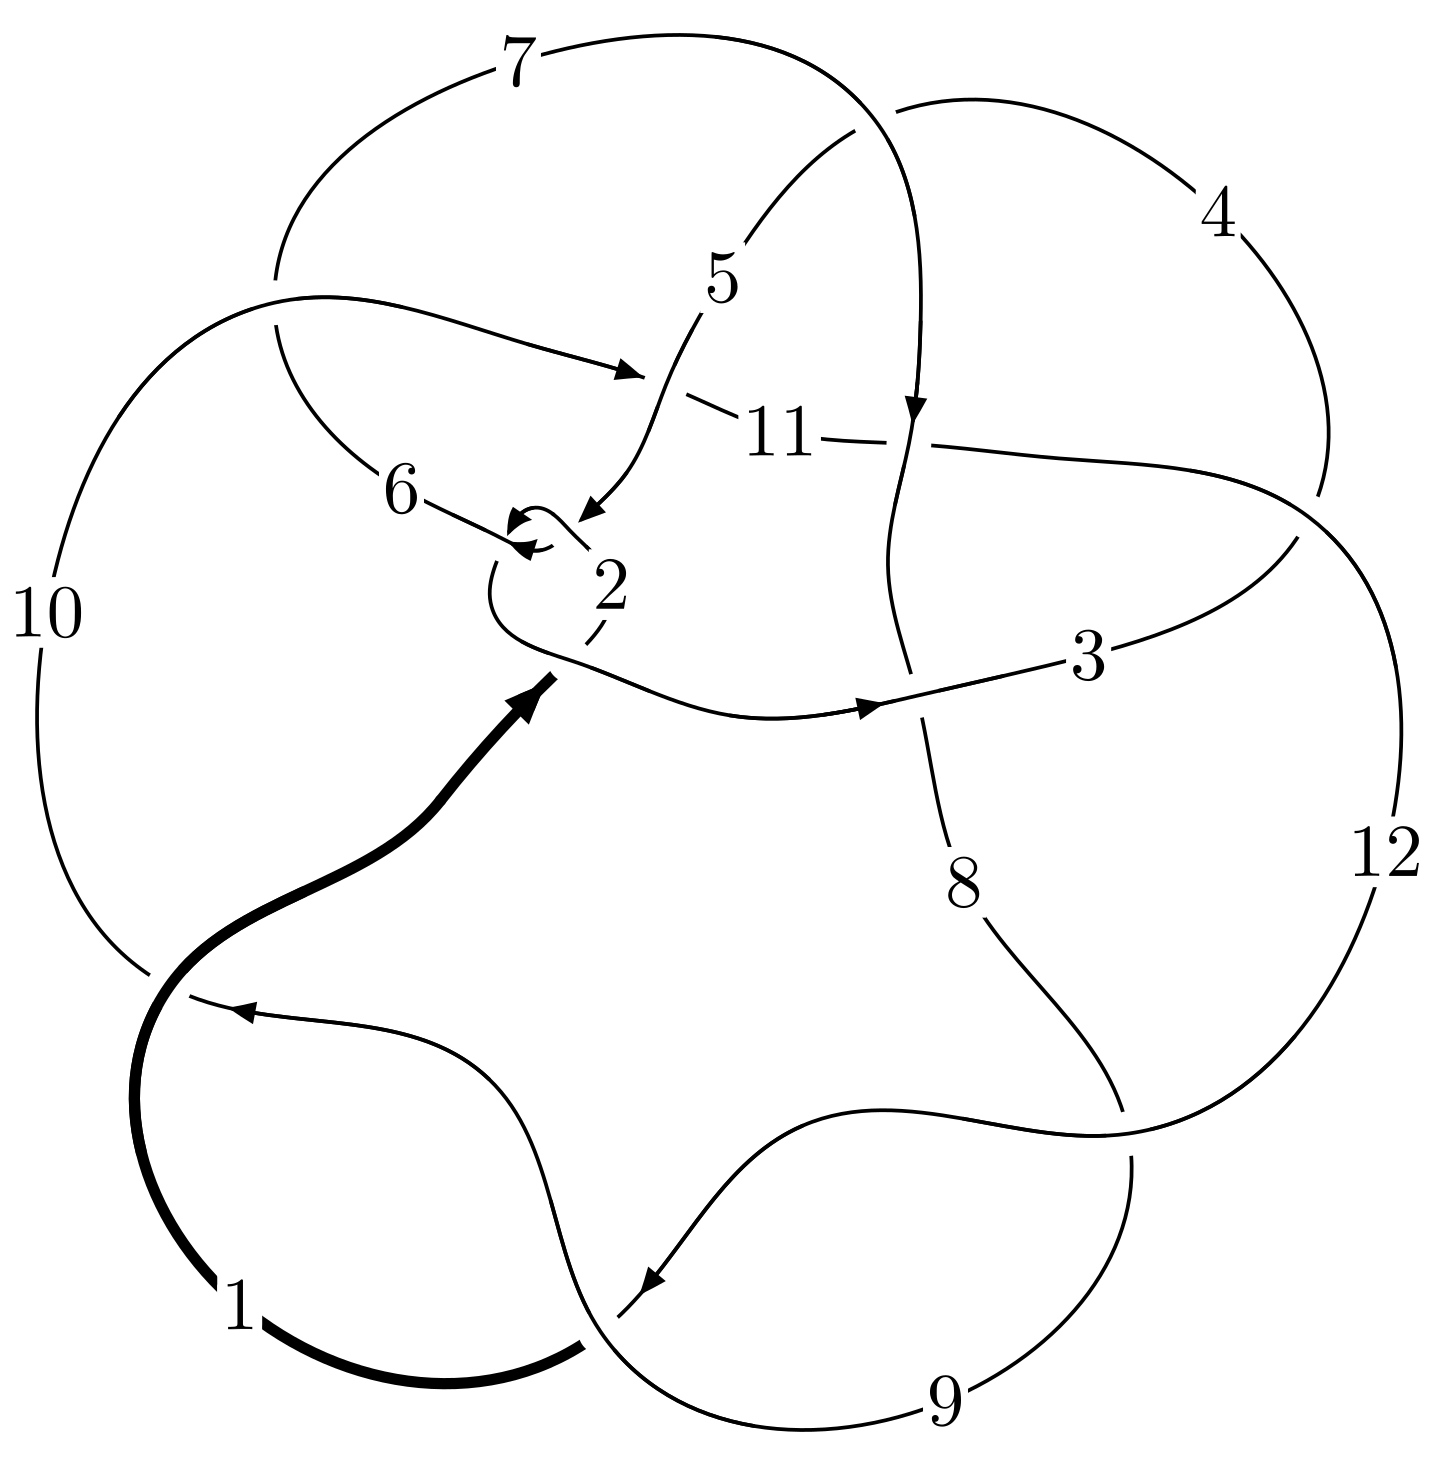
\includegraphics[width=112pt]{../../../GIT/diagram.site/Diagrams/png/2405_12n_0316.png}\\
\ \ \ A knot diagram\footnotemark}&
\allowdisplaybreaks
\textbf{Linearized knot diagam} \\
\cline{2-2}
 &
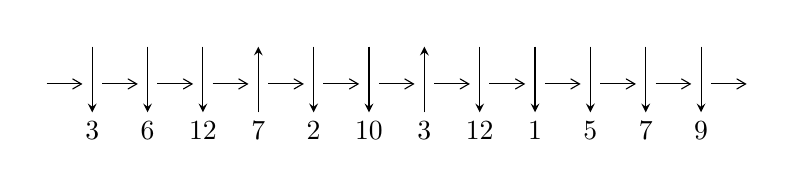
\begin{tikzpicture}[x=20pt, y=17pt]
	% nodes
	\node (C0) at (0, 0) {};
	\node (C1) at (1, 0) {};
	\node (C1U) at (1, +1) {};
	\node (C1D) at (1, -1) {3};

	\node (C2) at (2, 0) {};
	\node (C2U) at (2, +1) {};
	\node (C2D) at (2, -1) {6};

	\node (C3) at (3, 0) {};
	\node (C3U) at (3, +1) {};
	\node (C3D) at (3, -1) {12};

	\node (C4) at (4, 0) {};
	\node (C4U) at (4, +1) {};
	\node (C4D) at (4, -1) {7};

	\node (C5) at (5, 0) {};
	\node (C5U) at (5, +1) {};
	\node (C5D) at (5, -1) {2};

	\node (C6) at (6, 0) {};
	\node (C6U) at (6, +1) {};
	\node (C6D) at (6, -1) {10};

	\node (C7) at (7, 0) {};
	\node (C7U) at (7, +1) {};
	\node (C7D) at (7, -1) {3};

	\node (C8) at (8, 0) {};
	\node (C8U) at (8, +1) {};
	\node (C8D) at (8, -1) {12};

	\node (C9) at (9, 0) {};
	\node (C9U) at (9, +1) {};
	\node (C9D) at (9, -1) {1};

	\node (C10) at (10, 0) {};
	\node (C10U) at (10, +1) {};
	\node (C10D) at (10, -1) {5};

	\node (C11) at (11, 0) {};
	\node (C11U) at (11, +1) {};
	\node (C11D) at (11, -1) {7};

	\node (C12) at (12, 0) {};
	\node (C12U) at (12, +1) {};
	\node (C12D) at (12, -1) {9};
	\node (C13) at (13, 0) {};

	% arrows
	\draw[->,>={angle 60}]
	(C0) edge (C1) (C1) edge (C2) (C2) edge (C3) (C3) edge (C4) (C4) edge (C5) (C5) edge (C6) (C6) edge (C7) (C7) edge (C8) (C8) edge (C9) (C9) edge (C10) (C10) edge (C11) (C11) edge (C12) (C12) edge (C13) ;	\draw[->,>=stealth]
	(C1U) edge (C1D) (C2U) edge (C2D) (C3U) edge (C3D) (C4D) edge (C4U) (C5U) edge (C5D) (C6U) edge (C6D) (C7D) edge (C7U) (C8U) edge (C8D) (C9U) edge (C9D) (C10U) edge (C10D) (C11U) edge (C11D) (C12U) edge (C12D) ;
	\end{tikzpicture} \\
\hhline{~~} \\& 
\textbf{Solving Sequence} \\ \cline{2-2} 
 &
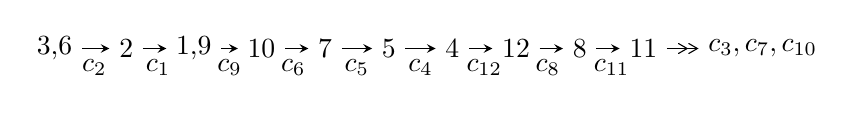
\begin{tikzpicture}[x=23pt, y=7pt]
	% node
	\node (A0) at (-1/8, 0) {3,6};
	\node (A1) at (1, 0) {2};
	\node (A2) at (33/16, 0) {1,9};
	\node (A3) at (25/8, 0) {10};
	\node (A4) at (33/8, 0) {7};
	\node (A5) at (41/8, 0) {5};
	\node (A6) at (49/8, 0) {4};
	\node (A7) at (57/8, 0) {12};
	\node (A8) at (65/8, 0) {8};
	\node (A9) at (73/8, 0) {11};
	\node (C1) at (1/2, -1) {$c_{2}$};
	\node (C2) at (3/2, -1) {$c_{1}$};
	\node (C3) at (21/8, -1) {$c_{9}$};
	\node (C4) at (29/8, -1) {$c_{6}$};
	\node (C5) at (37/8, -1) {$c_{5}$};
	\node (C6) at (45/8, -1) {$c_{4}$};
	\node (C7) at (53/8, -1) {$c_{12}$};
	\node (C8) at (61/8, -1) {$c_{8}$};
	\node (C9) at (69/8, -1) {$c_{11}$};
	\node (A10) at (11, 0) {$c_{3},c_{7},c_{10}$};

	% edge
	\draw[->,>=stealth]	
	(A0) edge (A1) (A1) edge (A2) (A2) edge (A3) (A3) edge (A4) (A4) edge (A5) (A5) edge (A6) (A6) edge (A7) (A7) edge (A8) (A8) edge (A9) ;
	\draw[->>,>={angle 60}]	
	(A9) edge (A10);
\end{tikzpicture} \\ 

\end{tabular} \\

\footnotetext{
The image of knot diagram is generated by the software ``\textbf{Draw programme}" developed by Andrew Bartholomew(\url{http://www.layer8.co.uk/maths/draw/index.htm\#Running-draw}), where we modified some parts for our purpose(\url{https://github.com/CATsTAILs/LinksPainter}).
}\phantom \\ \newline 
\centering \textbf{Ideals for irreducible components\footnotemark of $X_{\text{par}}$} 
 
\begin{align*}
I^u_{1}&=\langle 
1.49187\times10^{37} u^{44}-1.01328\times10^{37} u^{43}+\cdots+2.01007\times10^{37} b-7.03971\times10^{37},\\
\phantom{I^u_{1}}&\phantom{= \langle  }-1.39776\times10^{38} u^{44}+1.68461\times10^{38} u^{43}+\cdots+1.40705\times10^{38} a+1.95501\times10^{39},\\
\phantom{I^u_{1}}&\phantom{= \langle  }u^{45}-2 u^{44}+\cdots-63 u+7\rangle \\
I^u_{2}&=\langle 
-3 u^{12}-7 u^{11}+2 u^{10}+24 u^9+6 u^8-43 u^7-27 u^6+49 u^5+37 u^4-29 u^3-27 u^2+b+10 u+7,\\
\phantom{I^u_{2}}&\phantom{= \langle  }5 u^{12}+13 u^{11}-2 u^{10}-44 u^9-19 u^8+78 u^7+60 u^6-84 u^5-82 u^4+47 u^3+53 u^2+a-13 u-13,\\
\phantom{I^u_{2}}&\phantom{= \langle  }u^{13}+3 u^{12}+u^{11}-8 u^{10}-7 u^9+12 u^8+17 u^7-9 u^6-20 u^5+u^4+12 u^3+2 u^2-3 u-1\rangle \\
\\
\end{align*}
\raggedright * 2 irreducible components of $\dim_{\mathbb{C}}=0$, with total 58 representations.\\
\footnotetext{All coefficients of polynomials are rational numbers. But the coefficients are sometimes approximated in decimal forms when there is not enough margin.}
\newpage
\renewcommand{\arraystretch}{1}
\centering \section*{I. $I^u_{1}= \langle 1.49\times10^{37} u^{44}-1.01\times10^{37} u^{43}+\cdots+2.01\times10^{37} b-7.04\times10^{37},\;-1.40\times10^{38} u^{44}+1.68\times10^{38} u^{43}+\cdots+1.41\times10^{38} a+1.96\times10^{39},\;u^{45}-2 u^{44}+\cdots-63 u+7 \rangle$}
\flushleft \textbf{(i) Arc colorings}\\
\begin{tabular}{m{7pt} m{180pt} m{7pt} m{180pt} }
\flushright $a_{3}=$&$\begin{pmatrix}1\\0\end{pmatrix}$ \\
\flushright $a_{6}=$&$\begin{pmatrix}0\\u\end{pmatrix}$ \\
\flushright $a_{2}=$&$\begin{pmatrix}1\\- u^2\end{pmatrix}$ \\
\flushright $a_{1}=$&$\begin{pmatrix}- u^2+1\\- u^2\end{pmatrix}$ \\
\flushright $a_{9}=$&$\begin{pmatrix}0.993395 u^{44}-1.19726 u^{43}+\cdots+89.5674 u-13.8944\\-0.742197 u^{44}+0.504102 u^{43}+\cdots-24.9174 u+3.50222\end{pmatrix}$ \\
\flushright $a_{10}=$&$\begin{pmatrix}0.168633 u^{44}-0.289227 u^{43}+\cdots+40.1071 u-8.51481\\-0.625412 u^{44}+0.0300369 u^{43}+\cdots+0.0542180 u-0.00472178\end{pmatrix}$ \\
\flushright $a_{7}=$&$\begin{pmatrix}-2.57523 u^{44}+2.47327 u^{43}+\cdots-150.787 u+17.0513\\-0.238127 u^{44}-0.117959 u^{43}+\cdots+25.4258 u-2.94147\end{pmatrix}$ \\
\flushright $a_{5}=$&$\begin{pmatrix}u\\- u^3+u\end{pmatrix}$ \\
\flushright $a_{4}=$&$\begin{pmatrix}0.0434605 u^{44}-0.501873 u^{43}+\cdots+32.2099 u-4.00706\\-1.00696 u^{44}+1.07716 u^{43}+\cdots-66.0581 u+8.54528\end{pmatrix}$ \\
\flushright $a_{12}=$&$\begin{pmatrix}-1.44259 u^{44}+2.27648 u^{43}+\cdots-114.430 u+18.0623\\0.842298 u^{44}-0.861398 u^{43}+\cdots+32.9618 u-4.57062\end{pmatrix}$ \\
\flushright $a_{8}=$&$\begin{pmatrix}-2.81336 u^{44}+2.35531 u^{43}+\cdots-125.361 u+14.1099\\-0.238127 u^{44}-0.117959 u^{43}+\cdots+25.4258 u-2.94147\end{pmatrix}$ \\
\flushright $a_{11}=$&$\begin{pmatrix}-0.991831 u^{44}+1.08676 u^{43}+\cdots-88.6012 u+14.4109\\0.546953 u^{44}-0.100468 u^{43}+\cdots-0.832675 u-0.0412010\end{pmatrix}$\\&\end{tabular}
\flushleft \textbf{(ii) Obstruction class $= -1$}\\~\\
\flushleft \textbf{(iii) Cusp Shapes $= -1.33381 u^{44}+0.732754 u^{43}+\cdots-88.2937 u-0.929056$}\\~\\
\newpage\renewcommand{\arraystretch}{1}
\flushleft \textbf{(iv) u-Polynomials at the component}\newline \\
\begin{tabular}{m{50pt}|m{274pt}}
Crossings & \hspace{64pt}u-Polynomials at each crossing \\
\hline $$\begin{aligned}c_{1}\end{aligned}$$&$\begin{aligned}
&u^{45}+18 u^{44}+\cdots+3381 u+49
\end{aligned}$\\
\hline $$\begin{aligned}c_{2},c_{5}\end{aligned}$$&$\begin{aligned}
&u^{45}+2 u^{44}+\cdots-63 u-7
\end{aligned}$\\
\hline $$\begin{aligned}c_{3},c_{10}\end{aligned}$$&$\begin{aligned}
&u^{45}- u^{44}+\cdots-20 u-1
\end{aligned}$\\
\hline $$\begin{aligned}c_{4}\end{aligned}$$&$\begin{aligned}
&u^{45}+7 u^{44}+\cdots+15464 u+821
\end{aligned}$\\
\hline $$\begin{aligned}c_{6}\end{aligned}$$&$\begin{aligned}
&u^{45}+4 u^{44}+\cdots-22 u-4
\end{aligned}$\\
\hline $$\begin{aligned}c_{7}\end{aligned}$$&$\begin{aligned}
&u^{45}-3 u^{44}+\cdots+22696 u+3551
\end{aligned}$\\
\hline $$\begin{aligned}c_{8},c_{9},c_{12}\end{aligned}$$&$\begin{aligned}
&u^{45}+u^{44}+\cdots+64 u+19
\end{aligned}$\\
\hline $$\begin{aligned}c_{11}\end{aligned}$$&$\begin{aligned}
&u^{45}+u^{44}+\cdots-63 u+9
\end{aligned}$\\
\hline
\end{tabular}\\~\\
\newpage\renewcommand{\arraystretch}{1}
\flushleft \textbf{(v) Riley Polynomials at the component}\newline \\
\begin{tabular}{m{50pt}|m{274pt}}
Crossings & \hspace{64pt}Riley Polynomials at each crossing \\
\hline $$\begin{aligned}c_{1}\end{aligned}$$&$\begin{aligned}
&y^{45}+42 y^{44}+\cdots+6542725 y-2401
\end{aligned}$\\
\hline $$\begin{aligned}c_{2},c_{5}\end{aligned}$$&$\begin{aligned}
&y^{45}-18 y^{44}+\cdots+3381 y-49
\end{aligned}$\\
\hline $$\begin{aligned}c_{3},c_{10}\end{aligned}$$&$\begin{aligned}
&y^{45}+57 y^{44}+\cdots+198 y-1
\end{aligned}$\\
\hline $$\begin{aligned}c_{4}\end{aligned}$$&$\begin{aligned}
&y^{45}-63 y^{44}+\cdots+21028436 y-674041
\end{aligned}$\\
\hline $$\begin{aligned}c_{6}\end{aligned}$$&$\begin{aligned}
&y^{45}-4 y^{44}+\cdots-68 y-16
\end{aligned}$\\
\hline $$\begin{aligned}c_{7}\end{aligned}$$&$\begin{aligned}
&y^{45}-53 y^{44}+\cdots+550810170 y-12609601
\end{aligned}$\\
\hline $$\begin{aligned}c_{8},c_{9},c_{12}\end{aligned}$$&$\begin{aligned}
&y^{45}-35 y^{44}+\cdots-84 y-361
\end{aligned}$\\
\hline $$\begin{aligned}c_{11}\end{aligned}$$&$\begin{aligned}
&y^{45}+75 y^{44}+\cdots+405 y-81
\end{aligned}$\\
\hline
\end{tabular}\\~\\
\newpage\flushleft \textbf{(vi) Complex Volumes and Cusp Shapes}
$$\begin{array}{c|c|c}  
\text{Solutions to }I^u_{1}& \I (\text{vol} + \sqrt{-1}CS) & \text{Cusp shape}\\
 \hline 
\begin{aligned}
u &= -0.352517 + 0.930511 I \\
a &= -2.09255 - 0.56873 I \\
b &= -1.53917 - 0.68803 I\end{aligned}
 & \phantom{-}0.92371 - 3.61571 I & -7.30973 + 5.35358 I \\ \hline\begin{aligned}
u &= -0.352517 - 0.930511 I \\
a &= -2.09255 + 0.56873 I \\
b &= -1.53917 + 0.68803 I\end{aligned}
 & \phantom{-}0.92371 + 3.61571 I & -7.30973 - 5.35358 I \\ \hline\begin{aligned}
u &= -0.622969 + 0.745341 I \\
a &= -0.498948 - 0.274339 I \\
b &= \phantom{-}0.0307757 + 0.1234220 I\end{aligned}
 & \phantom{-}3.19833 + 0.47295 I & -2.90845 - 1.14935 I \\ \hline\begin{aligned}
u &= -0.622969 - 0.745341 I \\
a &= -0.498948 + 0.274339 I \\
b &= \phantom{-}0.0307757 - 0.1234220 I\end{aligned}
 & \phantom{-}3.19833 - 0.47295 I & -2.90845 + 1.14935 I \\ \hline\begin{aligned}
u &= \phantom{-}0.852606 + 0.644697 I \\
a &= -1.60431 + 2.03212 I \\
b &= -0.66092 + 1.63965 I\end{aligned}
 & \phantom{-}7.67151 - 0.54614 I & -7.14162 + 2.19289 I \\ \hline\begin{aligned}
u &= \phantom{-}0.852606 - 0.644697 I \\
a &= -1.60431 - 2.03212 I \\
b &= -0.66092 - 1.63965 I\end{aligned}
 & \phantom{-}7.67151 + 0.54614 I & -7.14162 - 2.19289 I \\ \hline\begin{aligned}
u &= \phantom{-}0.870374 + 0.636220 I \\
a &= -1.51114 + 2.96200 I \\
b &= \phantom{-}0.84979 + 1.64164 I\end{aligned}
 & \phantom{-}7.61467 - 4.45079 I & -7.29611 + 4.22653 I \\ \hline\begin{aligned}
u &= \phantom{-}0.870374 - 0.636220 I \\
a &= -1.51114 - 2.96200 I \\
b &= \phantom{-}0.84979 - 1.64164 I\end{aligned}
 & \phantom{-}7.61467 + 4.45079 I & -7.29611 - 4.22653 I \\ \hline\begin{aligned}
u &= -0.706985 + 0.572515 I \\
a &= \phantom{-}1.61320 + 1.43432 I \\
b &= \phantom{-}0.612546 + 1.273340 I\end{aligned}
 & -0.603650 + 1.183020 I & -7.09381 - 2.18131 I \\ \hline\begin{aligned}
u &= -0.706985 - 0.572515 I \\
a &= \phantom{-}1.61320 - 1.43432 I \\
b &= \phantom{-}0.612546 - 1.273340 I\end{aligned}
 & -0.603650 - 1.183020 I & -7.09381 + 2.18131 I\\
 \hline 
 \end{array}$$\newpage$$\begin{array}{c|c|c}  
\text{Solutions to }I^u_{1}& \I (\text{vol} + \sqrt{-1}CS) & \text{Cusp shape}\\
 \hline 
\begin{aligned}
u &= \phantom{-}1.017280 + 0.456940 I \\
a &= -0.20833 - 1.43339 I \\
b &= -1.77851 + 0.14760 I\end{aligned}
 & -2.41679 - 3.11933 I & -8.64263 + 5.00261 I \\ \hline\begin{aligned}
u &= \phantom{-}1.017280 - 0.456940 I \\
a &= -0.20833 + 1.43339 I \\
b &= -1.77851 - 0.14760 I\end{aligned}
 & -2.41679 + 3.11933 I & -8.64263 - 5.00261 I \\ \hline\begin{aligned}
u &= -0.837872 + 0.180212 I \\
a &= -0.719453 + 0.504755 I \\
b &= -0.475414 + 1.151620 I\end{aligned}
 & \phantom{-}5.23022 + 2.95335 I & -10.41493 - 5.15699 I \\ \hline\begin{aligned}
u &= -0.837872 - 0.180212 I \\
a &= -0.719453 - 0.504755 I \\
b &= -0.475414 - 1.151620 I\end{aligned}
 & \phantom{-}5.23022 - 2.95335 I & -10.41493 + 5.15699 I \\ \hline\begin{aligned}
u &= \phantom{-}0.829207 + 0.087175 I \\
a &= \phantom{-}2.10128 - 0.71672 I \\
b &= -0.375197 + 0.692927 I\end{aligned}
 & -6.31151 - 0.37732 I & -13.18619 - 0.42975 I \\ \hline\begin{aligned}
u &= \phantom{-}0.829207 - 0.087175 I \\
a &= \phantom{-}2.10128 + 0.71672 I \\
b &= -0.375197 - 0.692927 I\end{aligned}
 & -6.31151 + 0.37732 I & -13.18619 + 0.42975 I \\ \hline\begin{aligned}
u &= -0.780783 + 0.287291 I \\
a &= \phantom{-}0.16773 - 2.15348 I \\
b &= \phantom{-}1.01268 + 1.14500 I\end{aligned}
 & \phantom{-}5.58706 - 0.92954 I & -9.44375 - 1.95517 I \\ \hline\begin{aligned}
u &= -0.780783 - 0.287291 I \\
a &= \phantom{-}0.16773 + 2.15348 I \\
b &= \phantom{-}1.01268 - 1.14500 I\end{aligned}
 & \phantom{-}5.58706 + 0.92954 I & -9.44375 + 1.95517 I \\ \hline\begin{aligned}
u &= \phantom{-}0.741986 + 0.904888 I \\
a &= \phantom{-}1.232980 - 0.115587 I \\
b &= \phantom{-}0.350843 - 0.128409 I\end{aligned}
 & \phantom{-}12.46620 + 1.15235 I & -3.81779 + 0.34527 I \\ \hline\begin{aligned}
u &= \phantom{-}0.741986 - 0.904888 I \\
a &= \phantom{-}1.232980 + 0.115587 I \\
b &= \phantom{-}0.350843 + 0.128409 I\end{aligned}
 & \phantom{-}12.46620 - 1.15235 I & -3.81779 - 0.34527 I\\
 \hline 
 \end{array}$$\newpage$$\begin{array}{c|c|c}  
\text{Solutions to }I^u_{1}& \I (\text{vol} + \sqrt{-1}CS) & \text{Cusp shape}\\
 \hline 
\begin{aligned}
u &= -0.822383\phantom{ +0.000000I} \\
a &= -2.63142\phantom{ +0.000000I} \\
b &= \phantom{-}0.371288\phantom{ +0.000000I}\end{aligned}
 & -10.1445\phantom{ +0.000000I} & \phantom{-}9.33710\phantom{ +0.000000I} \\ \hline\begin{aligned}
u &= \phantom{-}0.702661 + 0.398793 I \\
a &= -0.853897 + 0.310274 I \\
b &= -0.210564 + 0.967639 I\end{aligned}
 & -1.09811 - 1.39547 I & -6.56054 + 4.96588 I \\ \hline\begin{aligned}
u &= \phantom{-}0.702661 - 0.398793 I \\
a &= -0.853897 - 0.310274 I \\
b &= -0.210564 - 0.967639 I\end{aligned}
 & -1.09811 + 1.39547 I & -6.56054 - 4.96588 I \\ \hline\begin{aligned}
u &= -1.021490 + 0.633982 I \\
a &= \phantom{-}0.047816 - 0.193328 I \\
b &= -0.358831 - 0.204765 I\end{aligned}
 & \phantom{-}1.97257 + 4.80081 I & -5.11482 - 5.89967 I \\ \hline\begin{aligned}
u &= -1.021490 - 0.633982 I \\
a &= \phantom{-}0.047816 + 0.193328 I \\
b &= -0.358831 + 0.204765 I\end{aligned}
 & \phantom{-}1.97257 - 4.80081 I & -5.11482 + 5.89967 I \\ \hline\begin{aligned}
u &= \phantom{-}0.760787 + 0.239478 I \\
a &= \phantom{-}0.429130 - 0.024508 I \\
b &= \phantom{-}0.810532 - 0.368894 I\end{aligned}
 & -1.101730 - 0.180700 I & -6.28342 - 1.85189 I \\ \hline\begin{aligned}
u &= \phantom{-}0.760787 - 0.239478 I \\
a &= \phantom{-}0.429130 + 0.024508 I \\
b &= \phantom{-}0.810532 + 0.368894 I\end{aligned}
 & -1.101730 + 0.180700 I & -6.28342 + 1.85189 I \\ \hline\begin{aligned}
u &= -1.067050 + 0.679768 I \\
a &= \phantom{-}0.77890 + 2.44088 I \\
b &= -0.89344 + 1.68496 I\end{aligned}
 & -1.81546 + 3.64143 I & -8.00000 - 2.52158 I \\ \hline\begin{aligned}
u &= -1.067050 - 0.679768 I \\
a &= \phantom{-}0.77890 - 2.44088 I \\
b &= -0.89344 - 1.68496 I\end{aligned}
 & -1.81546 - 3.64143 I & -8.00000 + 2.52158 I \\ \hline\begin{aligned}
u &= \phantom{-}1.018190 + 0.768985 I \\
a &= -0.662287 - 0.442499 I \\
b &= -0.108103 - 0.271060 I\end{aligned}
 & \phantom{-}11.57780 - 7.32875 I & -8.00000 + 4.62290 I\\
 \hline 
 \end{array}$$\newpage$$\begin{array}{c|c|c}  
\text{Solutions to }I^u_{1}& \I (\text{vol} + \sqrt{-1}CS) & \text{Cusp shape}\\
 \hline 
\begin{aligned}
u &= \phantom{-}1.018190 - 0.768985 I \\
a &= -0.662287 + 0.442499 I \\
b &= -0.108103 + 0.271060 I\end{aligned}
 & \phantom{-}11.57780 + 7.32875 I & -8.00000 - 4.62290 I \\ \hline\begin{aligned}
u &= \phantom{-}0.583636 + 1.148450 I \\
a &= \phantom{-}2.23765 - 1.83947 I \\
b &= \phantom{-}1.60697 - 1.61313 I\end{aligned}
 & \phantom{-}8.75418 + 6.80607 I & -8.00000 - 4.07465 I \\ \hline\begin{aligned}
u &= \phantom{-}0.583636 - 1.148450 I \\
a &= \phantom{-}2.23765 + 1.83947 I \\
b &= \phantom{-}1.60697 + 1.61313 I\end{aligned}
 & \phantom{-}8.75418 - 6.80607 I & -8.00000 + 4.07465 I \\ \hline\begin{aligned}
u &= -1.161870 + 0.639019 I \\
a &= \phantom{-}0.16411 - 2.14514 I \\
b &= \phantom{-}1.88266 - 1.13204 I\end{aligned}
 & -1.49977 + 9.31425 I & \phantom{-0.000000 } 0 \\ \hline\begin{aligned}
u &= -1.161870 - 0.639019 I \\
a &= \phantom{-}0.16411 + 2.14514 I \\
b &= \phantom{-}1.88266 + 1.13204 I\end{aligned}
 & -1.49977 - 9.31425 I & \phantom{-0.000000 } 0 \\ \hline\begin{aligned}
u &= \phantom{-}1.041350 + 0.853737 I \\
a &= -0.50445 + 1.98666 I \\
b &= \phantom{-}0.433982 + 1.234590 I\end{aligned}
 & -4.65783 - 3.47814 I & \phantom{-0.000000 } 0 \\ \hline\begin{aligned}
u &= \phantom{-}1.041350 - 0.853737 I \\
a &= -0.50445 - 1.98666 I \\
b &= \phantom{-}0.433982 - 1.234590 I\end{aligned}
 & -4.65783 + 3.47814 I & \phantom{-0.000000 } 0 \\ \hline\begin{aligned}
u &= \phantom{-}1.38604\phantom{ +0.000000I} \\
a &= \phantom{-}0.478642\phantom{ +0.000000I} \\
b &= \phantom{-}2.27111\phantom{ +0.000000I}\end{aligned}
 & -5.50304\phantom{ +0.000000I} & -17.6960\phantom{ +0.000000I} \\ \hline\begin{aligned}
u &= \phantom{-}1.17910 + 0.78373 I \\
a &= \phantom{-}0.21212 - 2.72362 I \\
b &= -1.47078 - 1.85341 I\end{aligned}
 & \phantom{-}6.8143 - 13.6617 I & \phantom{-0.000000 } 0 \\ \hline\begin{aligned}
u &= \phantom{-}1.17910 - 0.78373 I \\
a &= \phantom{-}0.21212 + 2.72362 I \\
b &= -1.47078 + 1.85341 I\end{aligned}
 & \phantom{-}6.8143 + 13.6617 I & \phantom{-0.000000 } 0\\
 \hline 
 \end{array}$$\newpage$$\begin{array}{c|c|c}  
\text{Solutions to }I^u_{1}& \I (\text{vol} + \sqrt{-1}CS) & \text{Cusp shape}\\
 \hline 
\begin{aligned}
u &= -1.28910 + 0.63728 I \\
a &= \phantom{-}0.22407 + 2.43968 I \\
b &= -1.41146 + 2.05143 I\end{aligned}
 & -1.85160 + 3.71712 I & \phantom{-0.000000 } 0 \\ \hline\begin{aligned}
u &= -1.28910 - 0.63728 I \\
a &= \phantom{-}0.22407 - 2.43968 I \\
b &= -1.41146 - 2.05143 I\end{aligned}
 & -1.85160 - 3.71712 I & \phantom{-0.000000 } 0 \\ \hline\begin{aligned}
u &= -1.10756 + 0.93089 I \\
a &= \phantom{-}0.042729 + 1.301160 I \\
b &= -0.474464 + 0.759384 I\end{aligned}
 & \phantom{-}0.57168 + 3.78059 I & \phantom{-0.000000 } 0 \\ \hline\begin{aligned}
u &= -1.10756 - 0.93089 I \\
a &= \phantom{-}0.042729 - 1.301160 I \\
b &= -0.474464 - 0.759384 I\end{aligned}
 & \phantom{-}0.57168 - 3.78059 I & \phantom{-0.000000 } 0 \\ \hline\begin{aligned}
u &= \phantom{-}0.138369\phantom{ +0.000000I} \\
a &= -2.03994\phantom{ +0.000000I} \\
b &= \phantom{-}0.689748\phantom{ +0.000000I}\end{aligned}
 & -0.867384\phantom{ +0.000000I} & -10.9880\phantom{ +0.000000I}\\
 \hline 
 \end{array}$$\newpage\newpage\renewcommand{\arraystretch}{1}
\centering \section*{II. $I^u_{2}= \langle -3 u^{12}-7 u^{11}+\cdots+b+7,\;5 u^{12}+13 u^{11}+\cdots+a-13,\;u^{13}+3 u^{12}+\cdots-3 u-1 \rangle$}
\flushleft \textbf{(i) Arc colorings}\\
\begin{tabular}{m{7pt} m{180pt} m{7pt} m{180pt} }
\flushright $a_{3}=$&$\begin{pmatrix}1\\0\end{pmatrix}$ \\
\flushright $a_{6}=$&$\begin{pmatrix}0\\u\end{pmatrix}$ \\
\flushright $a_{2}=$&$\begin{pmatrix}1\\- u^2\end{pmatrix}$ \\
\flushright $a_{1}=$&$\begin{pmatrix}- u^2+1\\- u^2\end{pmatrix}$ \\
\flushright $a_{9}=$&$\begin{pmatrix}-5 u^{12}-13 u^{11}+\cdots+13 u+13\\3 u^{12}+7 u^{11}+\cdots-10 u-7\end{pmatrix}$ \\
\flushright $a_{10}=$&$\begin{pmatrix}-6 u^{12}-15 u^{11}+\cdots+16 u+14\\5 u^{12}+12 u^{11}+\cdots-13 u-9\end{pmatrix}$ \\
\flushright $a_{7}=$&$\begin{pmatrix}-4 u^{12}-9 u^{11}+\cdots+8 u+3\\- u^{12}-3 u^{11}+\cdots- u+3\end{pmatrix}$ \\
\flushright $a_{5}=$&$\begin{pmatrix}u\\- u^3+u\end{pmatrix}$ \\
\flushright $a_{4}=$&$\begin{pmatrix}10 u^{12}+23 u^{11}+\cdots-25 u-13\\u^{12}+3 u^{11}+\cdots+2 u-4\end{pmatrix}$ \\
\flushright $a_{12}=$&$\begin{pmatrix}3 u^{12}+6 u^{11}+\cdots-8 u-8\\-6 u^{12}-15 u^{11}+\cdots+13 u+11\end{pmatrix}$ \\
\flushright $a_{8}=$&$\begin{pmatrix}-5 u^{12}-12 u^{11}+\cdots+7 u+6\\- u^{12}-3 u^{11}+\cdots- u+3\end{pmatrix}$ \\
\flushright $a_{11}=$&$\begin{pmatrix}-9 u^{12}-23 u^{11}+\cdots+23 u+20\\2 u^{12}+5 u^{11}+\cdots-6 u-4\end{pmatrix}$\\&\end{tabular}
\flushleft \textbf{(ii) Obstruction class $= 1$}\\~\\
\flushleft \textbf{(iii) Cusp Shapes $= 3 u^{12}+u^{11}-19 u^{10}-32 u^9+28 u^8+70 u^7-22 u^6-115 u^5-12 u^4+84 u^3+28 u^2-36 u-23$}\\~\\
\newpage\renewcommand{\arraystretch}{1}
\flushleft \textbf{(iv) u-Polynomials at the component}\newline \\
\begin{tabular}{m{50pt}|m{274pt}}
Crossings & \hspace{64pt}u-Polynomials at each crossing \\
\hline $$\begin{aligned}c_{1}\end{aligned}$$&$\begin{aligned}
&u^{13}-7 u^{12}+\cdots+13 u-1
\end{aligned}$\\
\hline $$\begin{aligned}c_{2}\end{aligned}$$&$\begin{aligned}
&u^{13}+3 u^{12}+\cdots-3 u-1
\end{aligned}$\\
\hline $$\begin{aligned}c_{3}\end{aligned}$$&$\begin{aligned}
&u^{13}+8 u^{11}+24 u^9+u^8+33 u^7+4 u^6+20 u^5+5 u^4+5 u^3+u^2+2 u-1
\end{aligned}$\\
\hline $$\begin{aligned}c_{4}\end{aligned}$$&$\begin{aligned}
&u^{13}+4 u^{11}+\cdots+6 u-1
\end{aligned}$\\
\hline $$\begin{aligned}c_{5}\end{aligned}$$&$\begin{aligned}
&u^{13}-3 u^{12}+\cdots-3 u+1
\end{aligned}$\\
\hline $$\begin{aligned}c_{6}\end{aligned}$$&$\begin{aligned}
&u^{13}+3 u^{12}-5 u^{10}+u^8-5 u^7+3 u^6+8 u^5- u^4-6 u^3- u^2+2 u+1
\end{aligned}$\\
\hline $$\begin{aligned}c_{7}\end{aligned}$$&$\begin{aligned}
&u^{13}+3 u^{11}+\cdots+6 u-1
\end{aligned}$\\
\hline $$\begin{aligned}c_{8},c_{9}\end{aligned}$$&$\begin{aligned}
&u^{13}-8 u^{11}+\cdots+2 u+1
\end{aligned}$\\
\hline $$\begin{aligned}c_{10}\end{aligned}$$&$\begin{aligned}
&u^{13}+8 u^{11}+24 u^9- u^8+33 u^7-4 u^6+20 u^5-5 u^4+5 u^3- u^2+2 u+1
\end{aligned}$\\
\hline $$\begin{aligned}c_{11}\end{aligned}$$&$\begin{aligned}
&u^{13}-2 u^{12}+\cdots-13 u-1
\end{aligned}$\\
\hline $$\begin{aligned}c_{12}\end{aligned}$$&$\begin{aligned}
&u^{13}-8 u^{11}+\cdots+2 u-1
\end{aligned}$\\
\hline
\end{tabular}\\~\\
\newpage\renewcommand{\arraystretch}{1}
\flushleft \textbf{(v) Riley Polynomials at the component}\newline \\
\begin{tabular}{m{50pt}|m{274pt}}
Crossings & \hspace{64pt}Riley Polynomials at each crossing \\
\hline $$\begin{aligned}c_{1}\end{aligned}$$&$\begin{aligned}
&y^{13}+21 y^{12}+\cdots+21 y-1
\end{aligned}$\\
\hline $$\begin{aligned}c_{2},c_{5}\end{aligned}$$&$\begin{aligned}
&y^{13}-7 y^{12}+\cdots+13 y-1
\end{aligned}$\\
\hline $$\begin{aligned}c_{3},c_{10}\end{aligned}$$&$\begin{aligned}
&y^{13}+16 y^{12}+\cdots+6 y-1
\end{aligned}$\\
\hline $$\begin{aligned}c_{4}\end{aligned}$$&$\begin{aligned}
&y^{13}+8 y^{12}+\cdots+4 y-1
\end{aligned}$\\
\hline $$\begin{aligned}c_{6}\end{aligned}$$&$\begin{aligned}
&y^{13}-9 y^{12}+\cdots+6 y-1
\end{aligned}$\\
\hline $$\begin{aligned}c_{7}\end{aligned}$$&$\begin{aligned}
&y^{13}+6 y^{12}+\cdots+22 y-1
\end{aligned}$\\
\hline $$\begin{aligned}c_{8},c_{9},c_{12}\end{aligned}$$&$\begin{aligned}
&y^{13}-16 y^{12}+\cdots+8 y-1
\end{aligned}$\\
\hline $$\begin{aligned}c_{11}\end{aligned}$$&$\begin{aligned}
&y^{13}-14 y^{12}+\cdots+29 y-1
\end{aligned}$\\
\hline
\end{tabular}\\~\\
\newpage\flushleft \textbf{(vi) Complex Volumes and Cusp Shapes}
$$\begin{array}{c|c|c}  
\text{Solutions to }I^u_{2}& \I (\text{vol} + \sqrt{-1}CS) & \text{Cusp shape}\\
 \hline 
\begin{aligned}
u &= -0.881035 + 0.428633 I \\
a &= -1.93807 - 2.18231 I \\
b &= \phantom{-}0.402497 - 1.355330 I\end{aligned}
 & -5.55501 + 1.76839 I & -9.42733 - 3.99027 I \\ \hline\begin{aligned}
u &= -0.881035 - 0.428633 I \\
a &= -1.93807 + 2.18231 I \\
b &= \phantom{-}0.402497 + 1.355330 I\end{aligned}
 & -5.55501 - 1.76839 I & -9.42733 + 3.99027 I \\ \hline\begin{aligned}
u &= \phantom{-}0.910742\phantom{ +0.000000I} \\
a &= \phantom{-}2.11436\phantom{ +0.000000I} \\
b &= -0.698976\phantom{ +0.000000I}\end{aligned}
 & -10.3385\phantom{ +0.000000I} & -32.2600\phantom{ +0.000000I} \\ \hline\begin{aligned}
u &= \phantom{-}0.988275 + 0.624685 I \\
a &= -0.18264 + 1.54866 I \\
b &= \phantom{-}0.822715 + 0.363964 I\end{aligned}
 & -4.28208 - 2.74184 I & -11.58472 + 0.68743 I \\ \hline\begin{aligned}
u &= \phantom{-}0.988275 - 0.624685 I \\
a &= -0.18264 - 1.54866 I \\
b &= \phantom{-}0.822715 - 0.363964 I\end{aligned}
 & -4.28208 + 2.74184 I & -11.58472 - 0.68743 I \\ \hline\begin{aligned}
u &= \phantom{-}0.786272 + 0.257302 I \\
a &= -1.165010 + 0.236660 I \\
b &= -0.544518 + 1.013380 I\end{aligned}
 & -1.90498 - 0.74935 I & -15.2105 + 0.6429 I \\ \hline\begin{aligned}
u &= \phantom{-}0.786272 - 0.257302 I \\
a &= -1.165010 - 0.236660 I \\
b &= -0.544518 - 1.013380 I\end{aligned}
 & -1.90498 + 0.74935 I & -15.2105 - 0.6429 I \\ \hline\begin{aligned}
u &= -1.010700 + 0.772169 I \\
a &= \phantom{-}0.445697 + 0.983245 I \\
b &= \phantom{-}0.008357 + 0.919135 I\end{aligned}
 & \phantom{-}1.40993 + 3.16875 I & -4.51782 - 0.85705 I \\ \hline\begin{aligned}
u &= -1.010700 - 0.772169 I \\
a &= \phantom{-}0.445697 - 0.983245 I \\
b &= \phantom{-}0.008357 - 0.919135 I\end{aligned}
 & \phantom{-}1.40993 - 3.16875 I & -4.51782 + 0.85705 I \\ \hline\begin{aligned}
u &= -0.501636 + 0.101564 I \\
a &= \phantom{-}0.96670 + 1.91810 I \\
b &= \phantom{-}0.581751 - 1.286380 I\end{aligned}
 & \phantom{-}6.06288 + 2.09354 I & -6.13746 - 2.14572 I\\
 \hline 
 \end{array}$$\newpage$$\begin{array}{c|c|c}  
\text{Solutions to }I^u_{2}& \I (\text{vol} + \sqrt{-1}CS) & \text{Cusp shape}\\
 \hline 
\begin{aligned}
u &= -0.501636 - 0.101564 I \\
a &= \phantom{-}0.96670 - 1.91810 I \\
b &= \phantom{-}0.581751 + 1.286380 I\end{aligned}
 & \phantom{-}6.06288 - 2.09354 I & -6.13746 + 2.14572 I \\ \hline\begin{aligned}
u &= -1.33655 + 1.04817 I \\
a &= \phantom{-}0.31613 + 3.50034 I \\
b &= -0.92132 + 3.01182 I\end{aligned}
 & -2.07604 + 4.55409 I & -12.9921 - 8.8615 I \\ \hline\begin{aligned}
u &= -1.33655 - 1.04817 I \\
a &= \phantom{-}0.31613 - 3.50034 I \\
b &= -0.92132 - 3.01182 I\end{aligned}
 & -2.07604 - 4.55409 I & -12.9921 + 8.8615 I\\
 \hline 
 \end{array}$$\newpage
\newpage\renewcommand{\arraystretch}{1}
\centering \section*{ III. u-Polynomials}
\begin{tabular}{m{50pt}|m{274pt}}
Crossings & \hspace{64pt}u-Polynomials at each crossing \\
\hline $$\begin{aligned}c_{1}\end{aligned}$$&$\begin{aligned}
&(u^{13}-7 u^{12}+\cdots+13 u-1)(u^{45}+18 u^{44}+\cdots+3381 u+49)
\end{aligned}$\\
\hline $$\begin{aligned}c_{2}\end{aligned}$$&$\begin{aligned}
&(u^{13}+3 u^{12}+\cdots-3 u-1)(u^{45}+2 u^{44}+\cdots-63 u-7)
\end{aligned}$\\
\hline $$\begin{aligned}c_{3}\end{aligned}$$&$\begin{aligned}
&(u^{13}+8 u^{11}+24 u^9+u^8+33 u^7+4 u^6+20 u^5+5 u^4+5 u^3+u^2+2 u-1)\\
&\cdot(u^{45}- u^{44}+\cdots-20 u-1)
\end{aligned}$\\
\hline $$\begin{aligned}c_{4}\end{aligned}$$&$\begin{aligned}
&(u^{13}+4 u^{11}+\cdots+6 u-1)(u^{45}+7 u^{44}+\cdots+15464 u+821)
\end{aligned}$\\
\hline $$\begin{aligned}c_{5}\end{aligned}$$&$\begin{aligned}
&(u^{13}-3 u^{12}+\cdots-3 u+1)(u^{45}+2 u^{44}+\cdots-63 u-7)
\end{aligned}$\\
\hline $$\begin{aligned}c_{6}\end{aligned}$$&$\begin{aligned}
&(u^{13}+3 u^{12}-5 u^{10}+u^8-5 u^7+3 u^6+8 u^5- u^4-6 u^3- u^2+2 u+1)\\
&\cdot(u^{45}+4 u^{44}+\cdots-22 u-4)
\end{aligned}$\\
\hline $$\begin{aligned}c_{7}\end{aligned}$$&$\begin{aligned}
&(u^{13}+3 u^{11}+\cdots+6 u-1)(u^{45}-3 u^{44}+\cdots+22696 u+3551)
\end{aligned}$\\
\hline $$\begin{aligned}c_{8},c_{9}\end{aligned}$$&$\begin{aligned}
&(u^{13}-8 u^{11}+\cdots+2 u+1)(u^{45}+u^{44}+\cdots+64 u+19)
\end{aligned}$\\
\hline $$\begin{aligned}c_{10}\end{aligned}$$&$\begin{aligned}
&(u^{13}+8 u^{11}+24 u^9- u^8+33 u^7-4 u^6+20 u^5-5 u^4+5 u^3- u^2+2 u+1)\\
&\cdot(u^{45}- u^{44}+\cdots-20 u-1)
\end{aligned}$\\
\hline $$\begin{aligned}c_{11}\end{aligned}$$&$\begin{aligned}
&(u^{13}-2 u^{12}+\cdots-13 u-1)(u^{45}+u^{44}+\cdots-63 u+9)
\end{aligned}$\\
\hline $$\begin{aligned}c_{12}\end{aligned}$$&$\begin{aligned}
&(u^{13}-8 u^{11}+\cdots+2 u-1)(u^{45}+u^{44}+\cdots+64 u+19)
\end{aligned}$\\
\hline
\end{tabular}\newpage\renewcommand{\arraystretch}{1}
\centering \section*{ IV. Riley Polynomials}
\begin{tabular}{m{50pt}|m{274pt}}
Crossings & \hspace{64pt}Riley Polynomials at each crossing \\
\hline $$\begin{aligned}c_{1}\end{aligned}$$&$\begin{aligned}
&(y^{13}+21 y^{12}+\cdots+21 y-1)(y^{45}+42 y^{44}+\cdots+6542725 y-2401)
\end{aligned}$\\
\hline $$\begin{aligned}c_{2},c_{5}\end{aligned}$$&$\begin{aligned}
&(y^{13}-7 y^{12}+\cdots+13 y-1)(y^{45}-18 y^{44}+\cdots+3381 y-49)
\end{aligned}$\\
\hline $$\begin{aligned}c_{3},c_{10}\end{aligned}$$&$\begin{aligned}
&(y^{13}+16 y^{12}+\cdots+6 y-1)(y^{45}+57 y^{44}+\cdots+198 y-1)
\end{aligned}$\\
\hline $$\begin{aligned}c_{4}\end{aligned}$$&$\begin{aligned}
&(y^{13}+8 y^{12}+\cdots+4 y-1)(y^{45}-63 y^{44}+\cdots+2.10284\times10^{7} y-674041)
\end{aligned}$\\
\hline $$\begin{aligned}c_{6}\end{aligned}$$&$\begin{aligned}
&(y^{13}-9 y^{12}+\cdots+6 y-1)(y^{45}-4 y^{44}+\cdots-68 y-16)
\end{aligned}$\\
\hline $$\begin{aligned}c_{7}\end{aligned}$$&$\begin{aligned}
&(y^{13}+6 y^{12}+\cdots+22 y-1)\\
&\cdot(y^{45}-53 y^{44}+\cdots+550810170 y-12609601)
\end{aligned}$\\
\hline $$\begin{aligned}c_{8},c_{9},c_{12}\end{aligned}$$&$\begin{aligned}
&(y^{13}-16 y^{12}+\cdots+8 y-1)(y^{45}-35 y^{44}+\cdots-84 y-361)
\end{aligned}$\\
\hline $$\begin{aligned}c_{11}\end{aligned}$$&$\begin{aligned}
&(y^{13}-14 y^{12}+\cdots+29 y-1)(y^{45}+75 y^{44}+\cdots+405 y-81)
\end{aligned}$\\
\hline
\end{tabular}
\vskip 2pc
\end{document}